%% ============================================================
%% 分片 18：原文第 6 节「Loop and Line Operators」（原文 glshort.tex 起于第 4483 行）
%% 由 tools/harvmac2tex.py 从 arXiv 源码（hep-th/0604151v3）自动生成。
%% 只译英文散文；公式、编号、\label、\cite 一律不改。
%% ============================================================

\subsection{Line Operator Near A Boundary}

\label{sec:lineop}

The geometric Langlands program revolves around the case that
$\Sigma$ has a boundary and the line operator  runs parallel to
the boundary.

\begin{figure}[htbp]
\centering
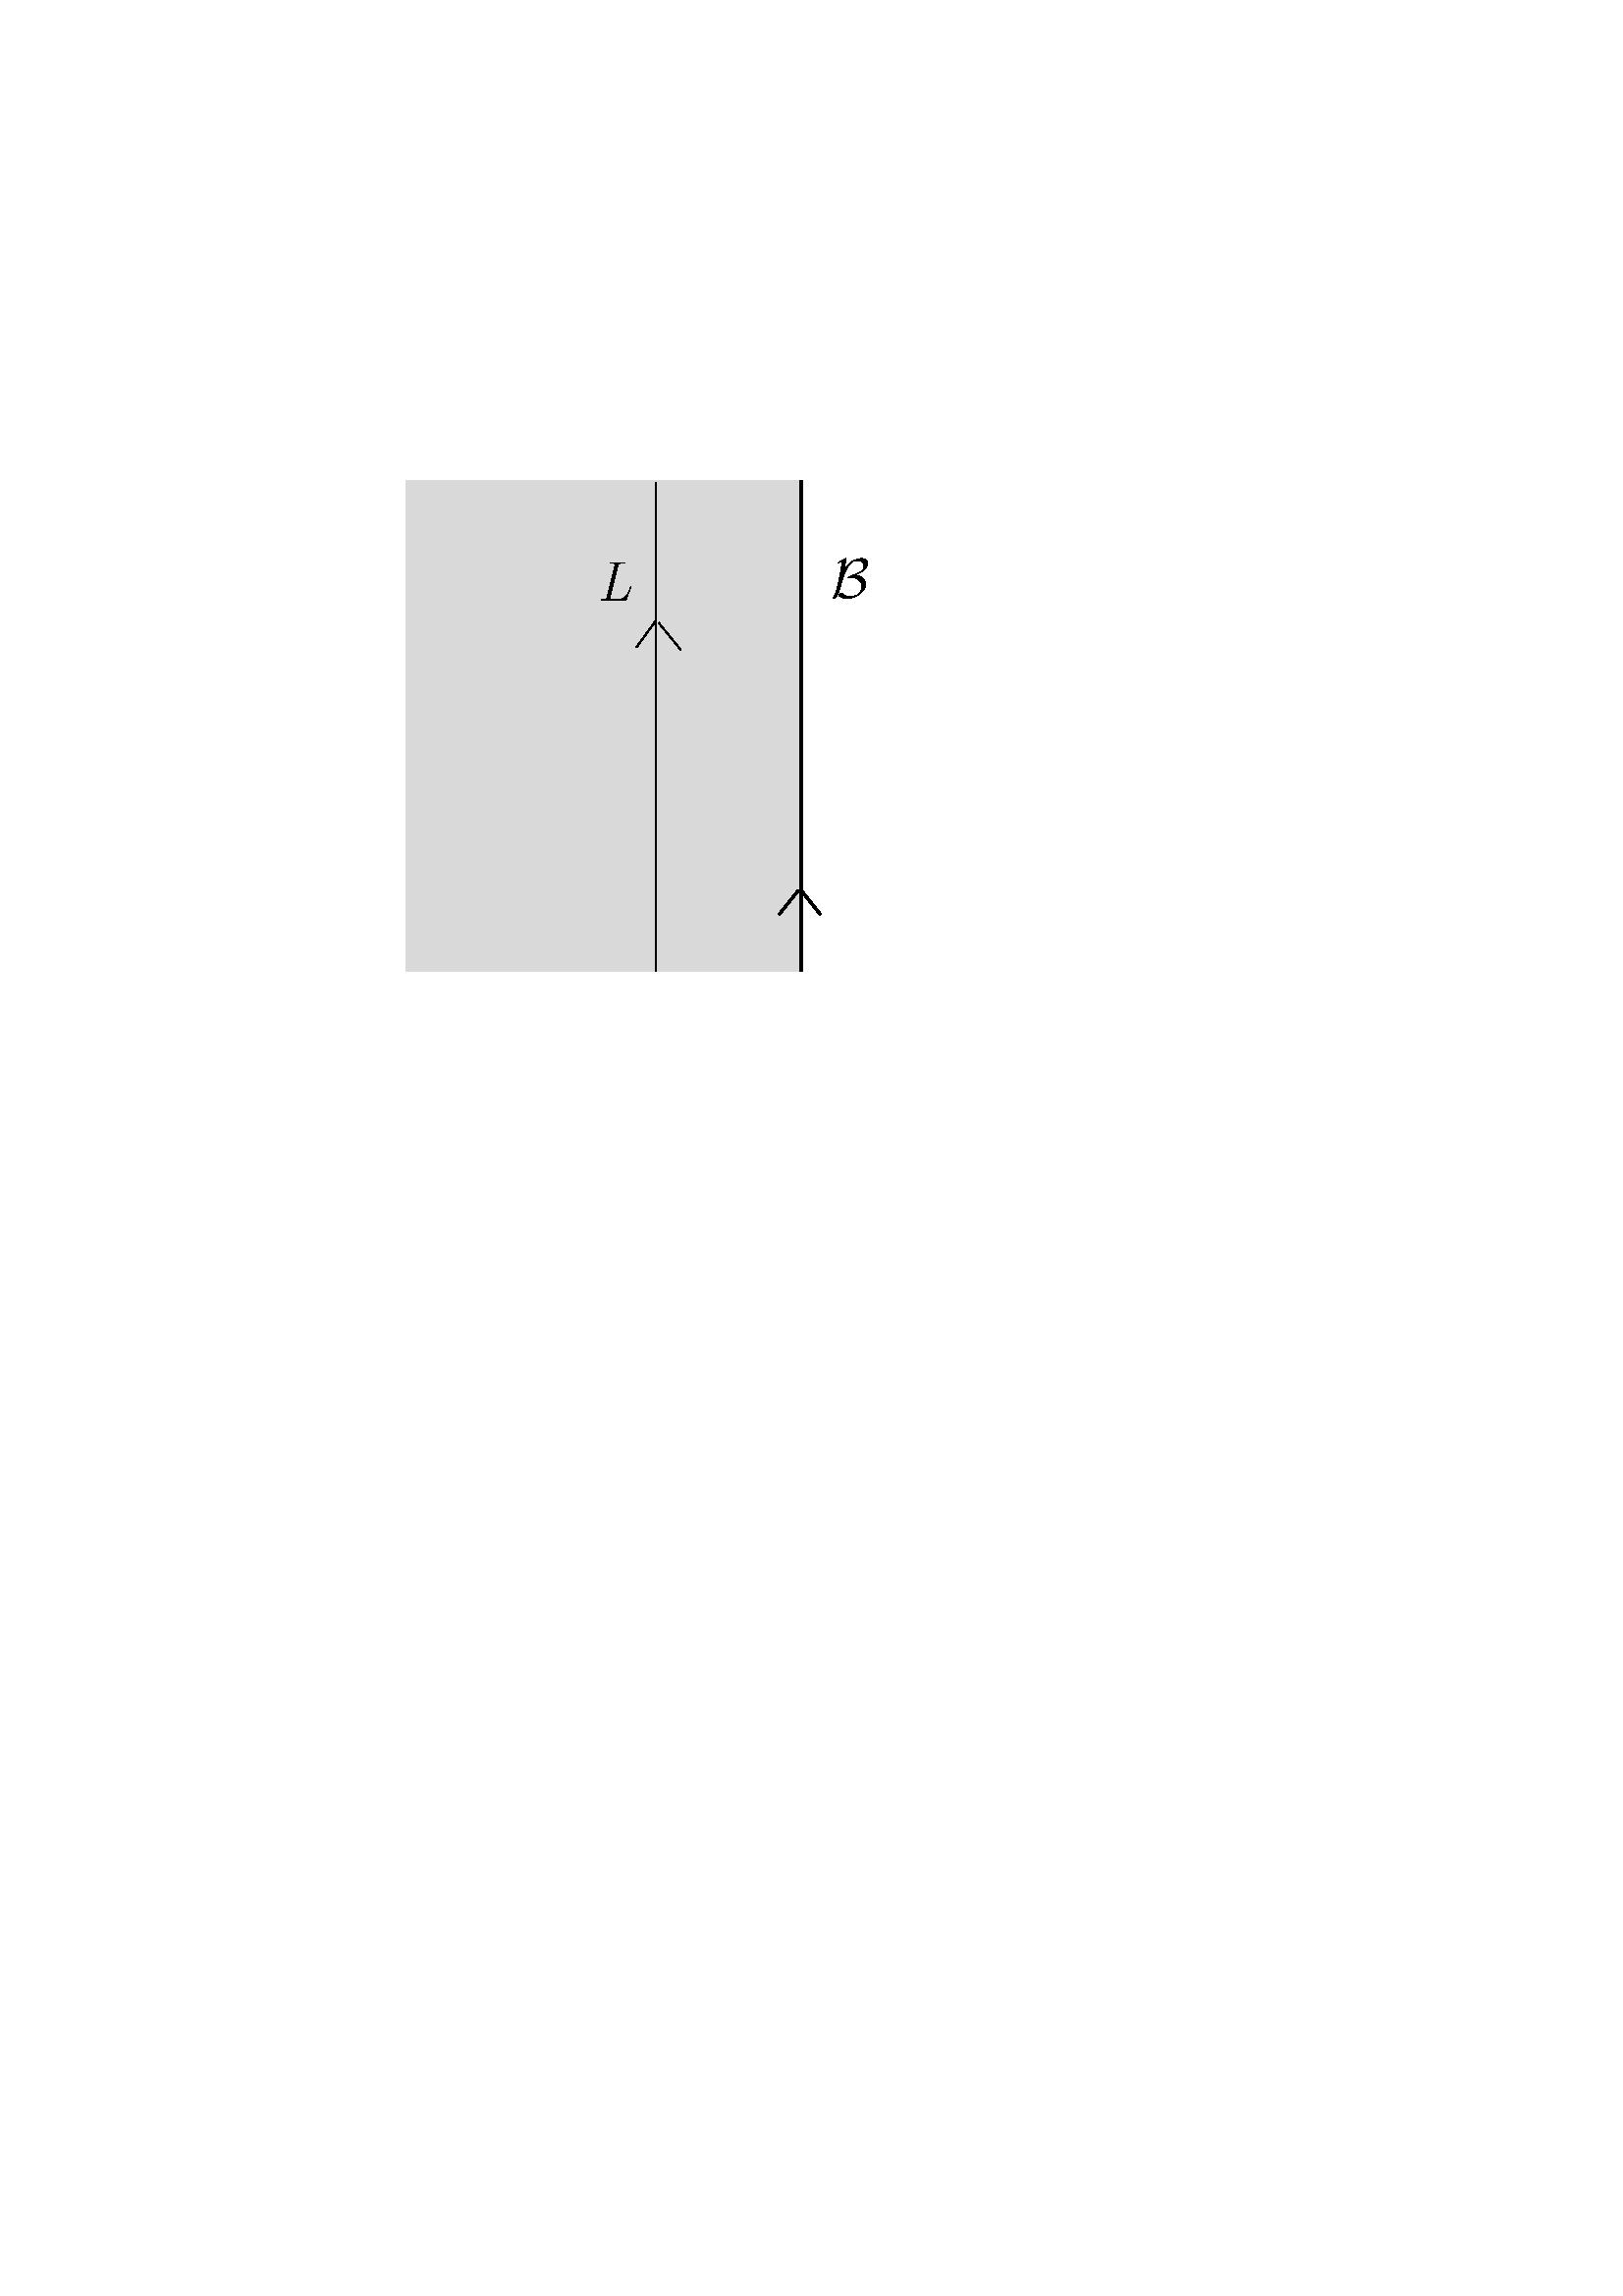
\includegraphics[width=0.75\linewidth]{figures/gla4-4.png}
\caption{A Riemann surface with a boundary, labeled by a brane ${\cal B}$, and a line operator $L$ parallel to the boundary.（原文 Fig.~7）}
\label{fig:trinamp}
\end{figure}

 Defining a quantum field theory on the Riemann surface $\Sigma$
with boundary requires a choice of boundary condition -- that is a
choice of a brane, which we will call ${\cal B}$. In \trinamp, we
sketch a Riemann surface $\Sigma $ with a boundary and a line $L$
parallel to the boundary. The boundary has been labeled by a brane
${\cal B}$, which defines the boundary conditions at that
boundary. A line operator $\EUX$ is supported on $L$. $\EUX$ may
be a Wilson, 't Hooft, or mixed Wilson-'t Hooft operator.

{}From a macroscopic point of view,  $\EUX$ and ${\cal B}$ simply
combine together into an effective boundary condition ${\cal B}'$.
One can characterize ${\cal B}'$ as the effective boundary
condition that one sees at a big distance due to the combined
effects of ${\cal B}$ and $\EUX$. Or one can simply take the limit
that $L$ approaches the boundary and let ${\cal B}'$ be the
limiting boundary condition that results.

Either way, we write ${\cal B}'=\EUX {\cal B}$ for the new brane
that is produced by acting with $\EUX$ on the old brane.   In this
way, we regard line operators as acting on boundary conditions to
produce new boundary conditions.

\begin{figure}[htbp]
\centering
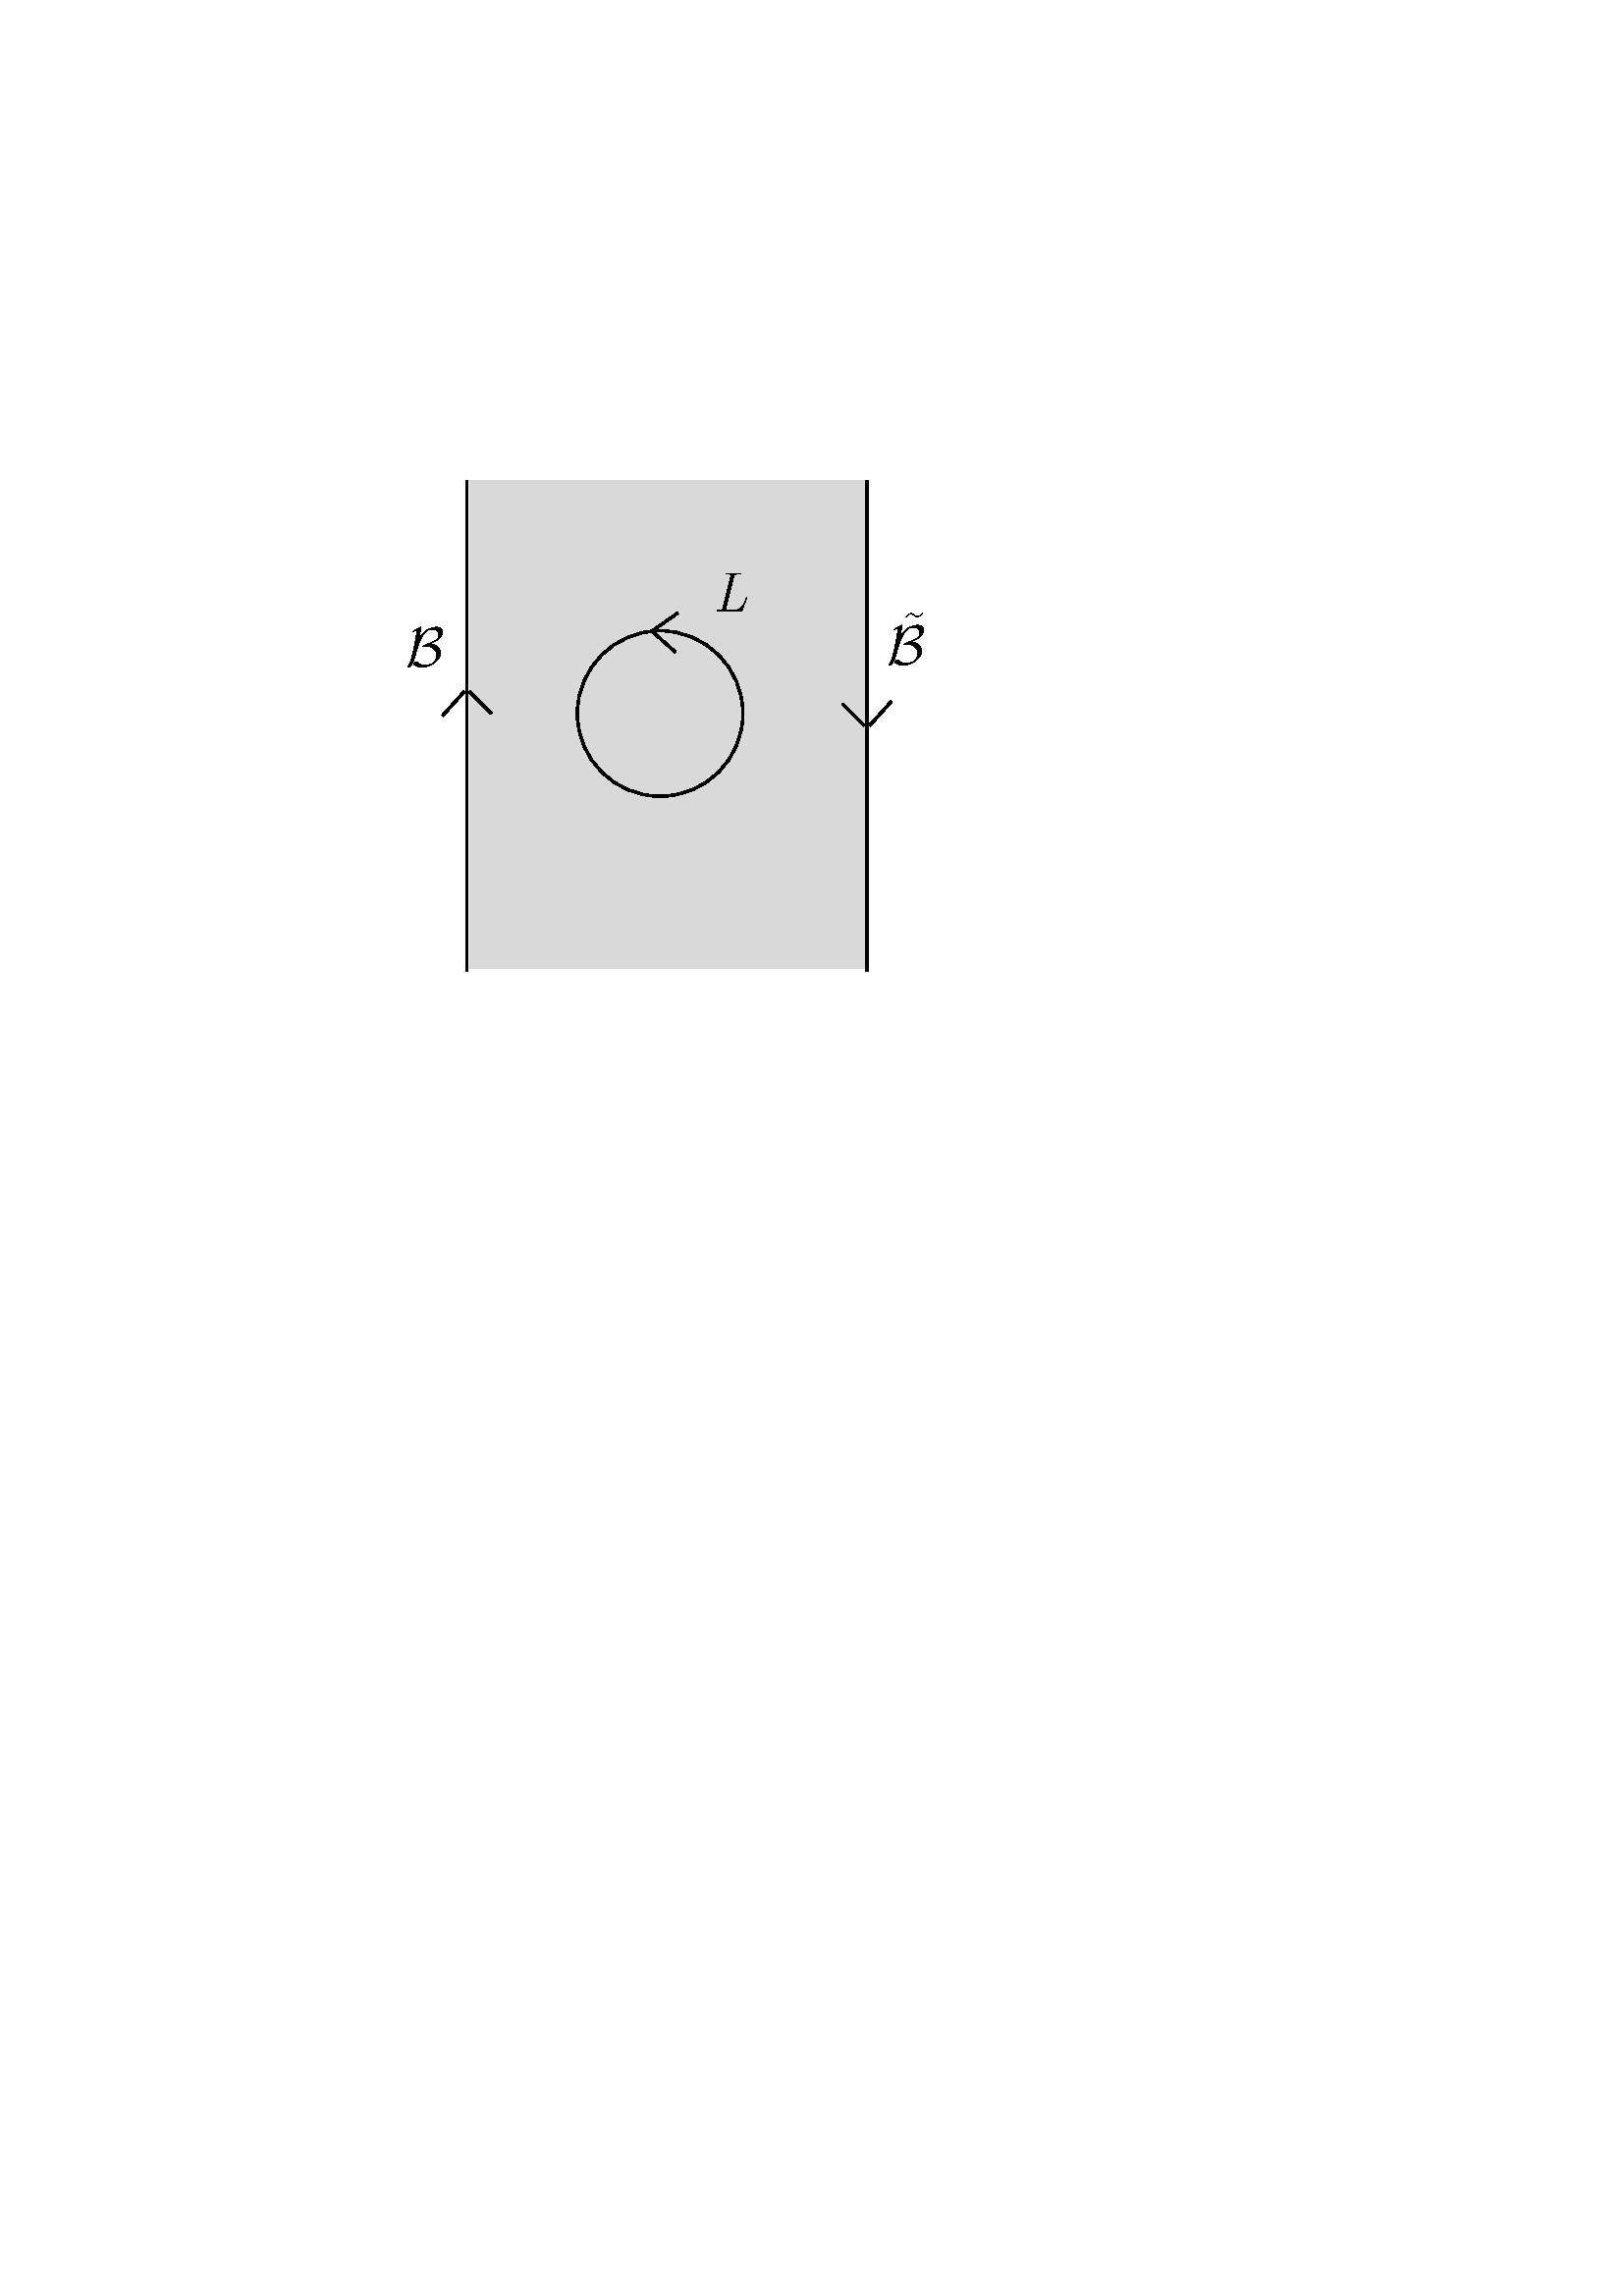
\includegraphics[width=0.75\linewidth]{figures/gla4-5.png}
\caption{Action of a loop operator as an ordinary operator on the space ${\cal H}_{\cal B,\tilde{\cal B}}$.（原文 Fig.~8）}
\label{fig:quadramp}
\end{figure}
 This is a more abstract form
of action than the usual action of an operator on a vector space.
As we saw above, to get a  vector space ${\cal H}_{{\cal B},\tilde
{\cal B}}$ associated with ${\cal B}$ on which an operator  might
act, we need a pair of branes ${\cal B}$ and  $\tilde {\cal B}$.
Of course, we can just take $\tilde {\cal B}={\cal B}$. But even
once we construct a space ${\cal H}_{{\cal B},\tilde {\cal B}}$ of
physical states, it is really a {\it loop} operator, localized in
time, that acts on this space, by quantizing the picture of
\quadramp. An open line operator that runs in the time direction,
as in \trinamp, is instead part of the data that must be
incorporated in quantization to get the right space of physical
states.

If we {\it do} have a vector space ${\cal H}$ and an operator
${\EUO}:{\cal H}\to {\cal H}$, we can look for a vector $\psi\in
{\cal H}$ that is an eigenvector of ${\EUO}$:
% 式 (6.21)
\setcounter{equation}{20}
\begin{equation}\label{eq:reot}
{\EUO}\psi=\lambda\psi.
\end{equation}
 Here $\lambda$ is an ordinary
complex number.

In our problem, instead of an operator that acts on vectors in a
Hilbert space, we have a more exotic operator that acts on
theories, via ${\cal B}\to {\cal B}'=\EUX {\cal B}$.   An ordinary
complex eigenvalue does not make sense in this situation. Rather,
what plays the role of an ``eigenvalue'' is a vector space $V$.

For every brane ${\cal B}$ and vector space $V$, one defines a new
brane ${\cal B}\otimes V$.  An abstract way to characterize ${\cal
B}\otimes V$ is to say that for any brane $\tilde {\cal B}$, the
Hilbert space ${\cal H}_{\tilde {\cal B},{\cal B}\otimes V}$ is
equal to ${\cal H}_{\tilde {\cal B}, {\cal B}}\otimes V$.

We can be more concrete in the case of branes that are constructed
from geometry.  In the case that theory $X$ is a two-dimensional
sigma-model with a target space $\hat X$, a brane can be
constructed from a vector bundle ${\cal W}\to \hat X$ (or from a
more general sheaf, possibly suported on a submanifold). ${\cal
W}$ is known as the Chan-Paton bundle. Tensoring such a brane with
a fixed vector space $V$ just means replacing ${\cal W}$ by ${\cal
W}\otimes V$. This operation generalizes without any problem when
${\cal W}$ is replaced by a more general sheaf.

If we identify $V$ as $\Bbb{C}^k$ for some $k$, then tensoring the
Chan-Paton bundle with $V$ amounts to taking $k$ copies of the
original brane. So for ${\cal B}$ to be an eigenbrane for $\EUX$
means that $\EUX{\cal B}$ is isomorphic to the sum of $k$ copies
of ${\cal B}$.  However, it is much better to think of the
``eigenvalue'' as a vector space $V$, not just its integer
dimension $k$, since $V$ may in fact vary with some additional
parameters as the fiber of a vector bundle over some parameter
space.

Having established the notion of tensoring a brane by a vector
space, we now can define the  notion of eigenbrane.  A brane
${\cal B}$ is an eigenbrane for a line operator $\EUX$ if
% 式 (6.22)
\setcounter{equation}{21}
\begin{equation}\label{eq:intico}
\EUX {\cal B}={\cal B}\otimes V,
\end{equation}
 for some vector
space $V$.  This concept corresponds to the concept of an
eigensheaf as defined by Beilinson and Drinfeld in the geometric
Langlands program \cite{ref5}.

\begin{figure}[htbp]
\centering
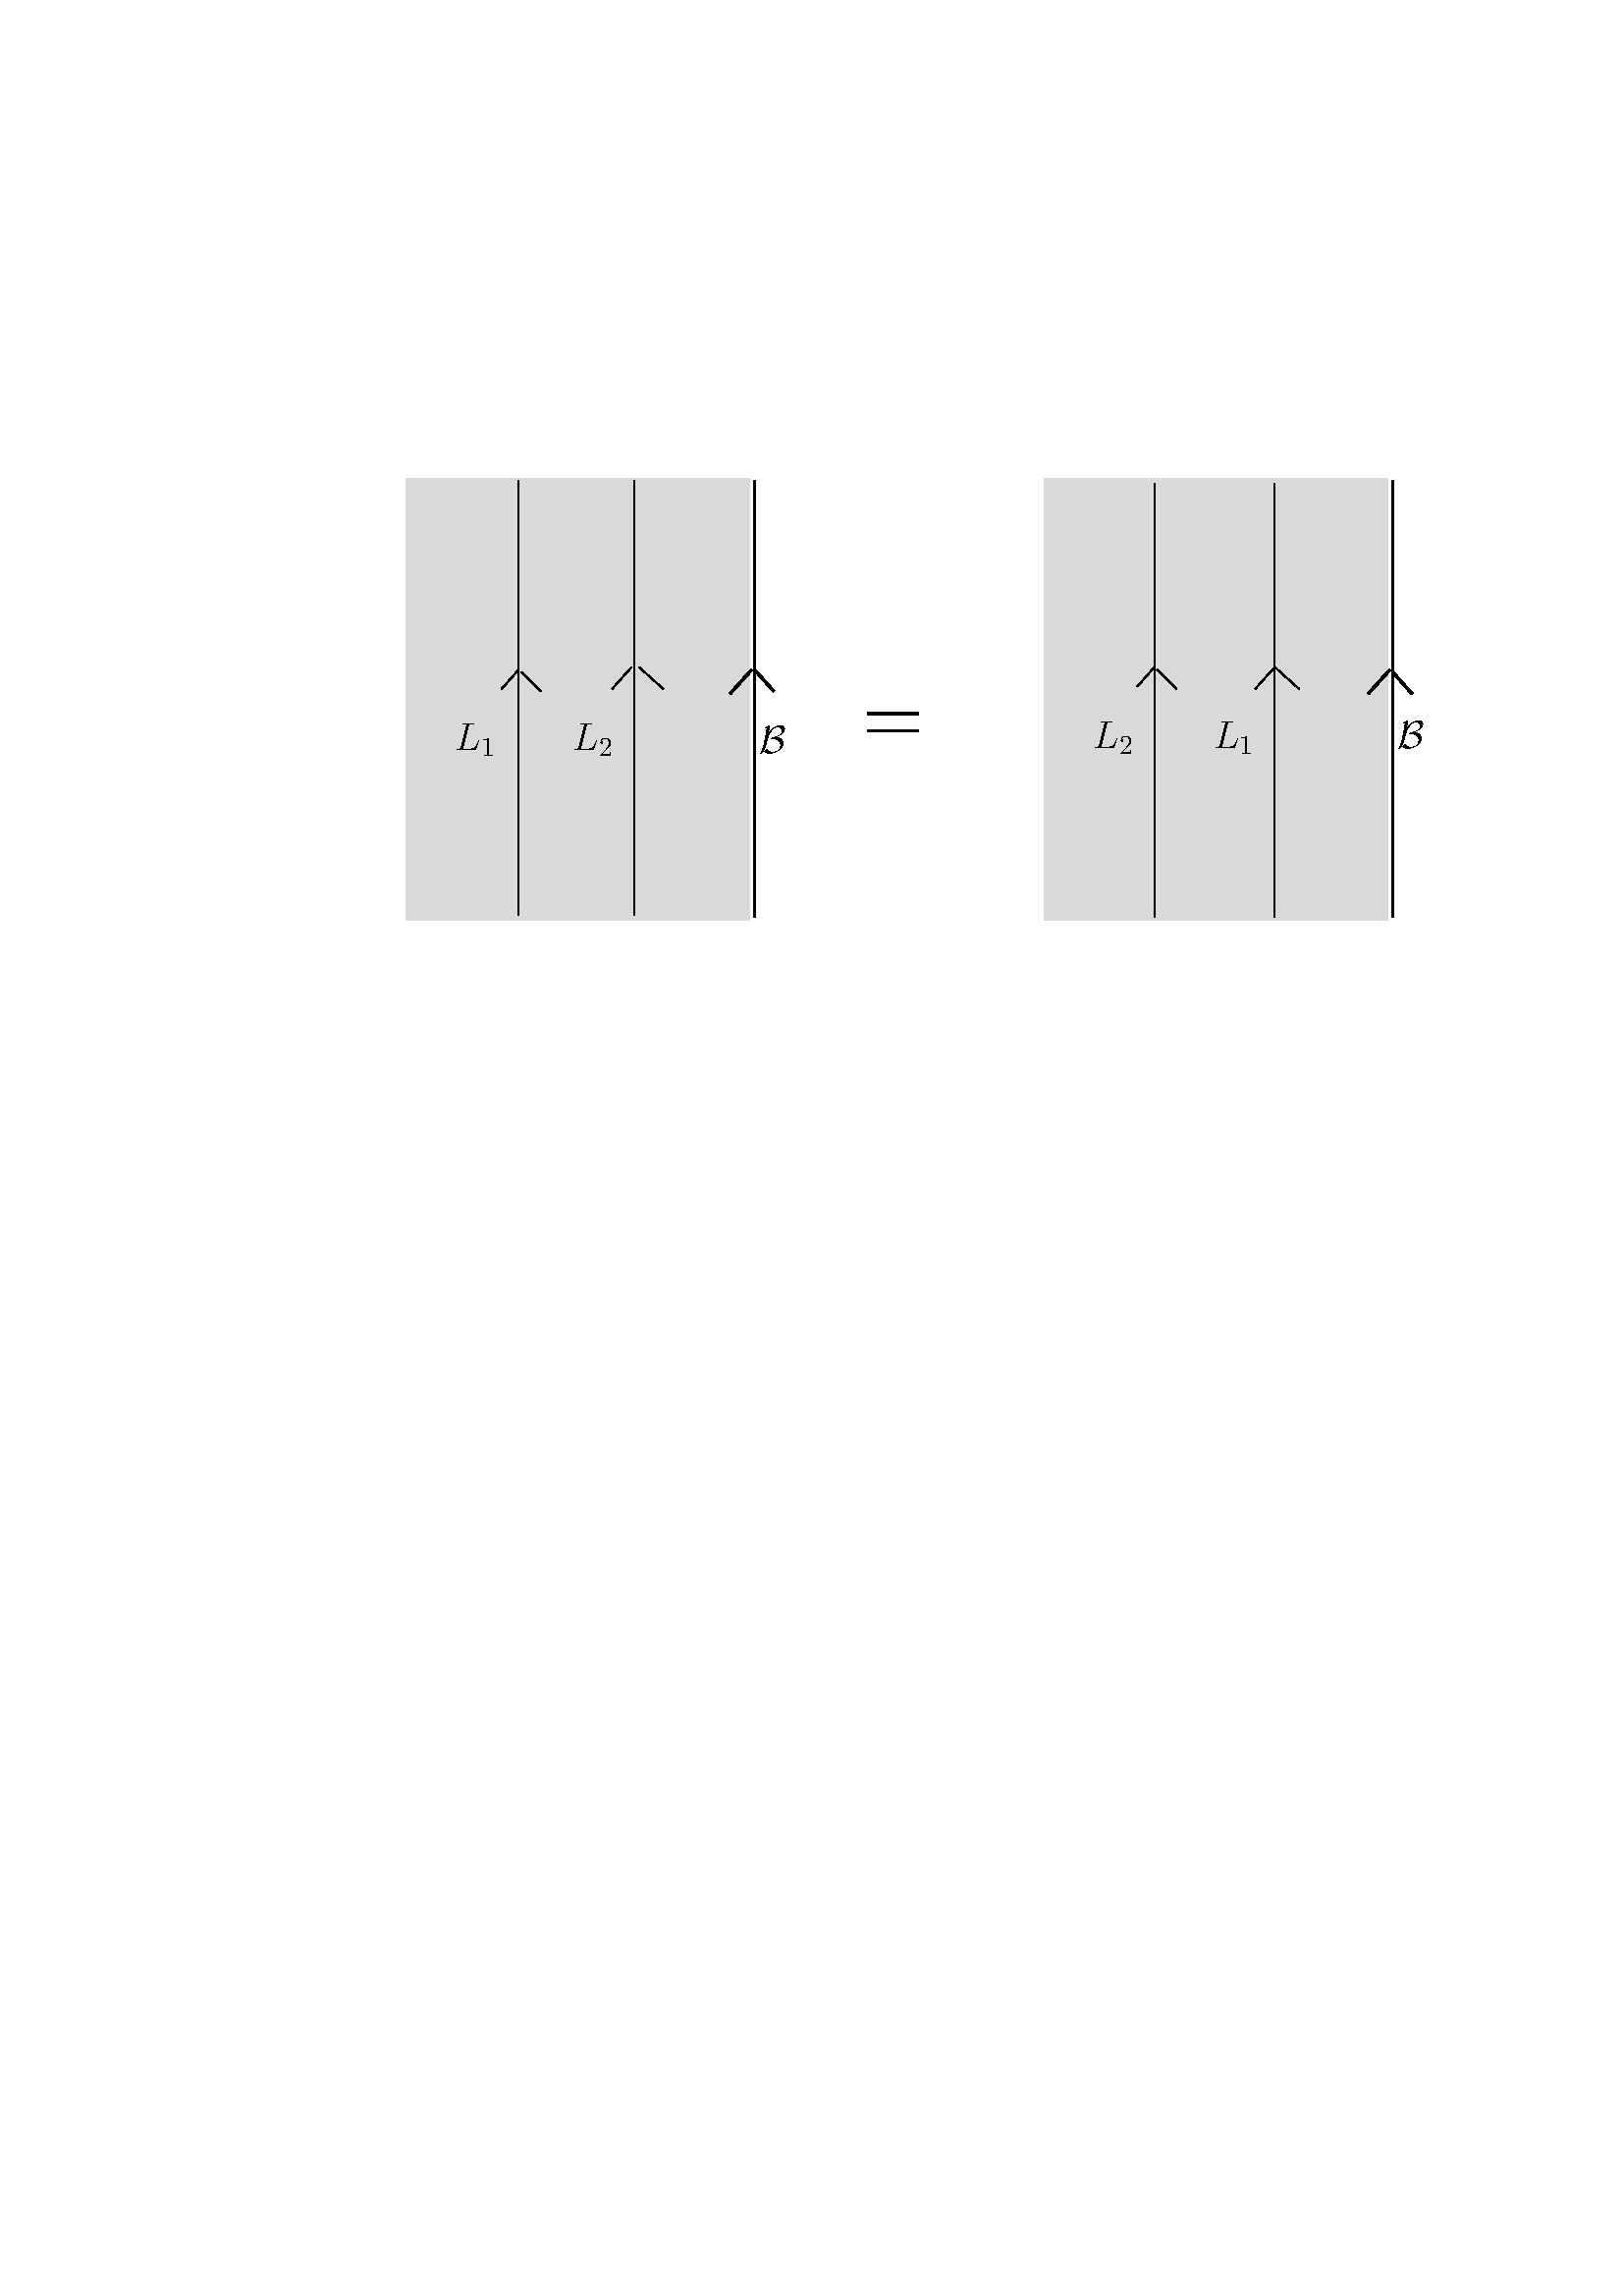
\includegraphics[width=0.75\linewidth]{figures/gla4-6.png}
\caption{Line operators $L_1$ and $L_2$ are said to commute if they can be passed through each other without singularity. In topological field theory, this simply means that the two figures pictured here can be considered equivalent.（原文 Fig.~9）}
\label{fig:quintamp}
\end{figure}
 If $\EUX_1$ and $\EUX_2$ are
two line operators, supported on parallel lines $L_1$ and $L_2$,
we say that they commute if for all ${\cal B}$ we have
% 式 (6.23)
\setcounter{equation}{22}
\begin{equation}\label{eq:pintico}
\EUX_1\EUX_2{\cal B}=\EUX_2\EUX_1{\cal B}.
\end{equation}
 This
statement can be illustrated in a convenient picture: it means
that the lines $L_1$ and $L_2$  can be passed through each other
without any discontinuity (\quintamp). Just as for ordinary
operators on a Hilbert space, if two line operators commute in
this sense, it is possible for them to have a simultaneous
eigenbrane, that is, a brane ${\cal B}$ obeying:
% [WARN] 公式 \eqn\eqref{eq:pintico} 无编号或重复
\begin{equation*}
\tag*{(6.24)}
\begin{aligned}\EUX_1{\cal B}& = {\cal B}\otimes V_1\\
\EUX_2{\cal B}& = {\cal B}\otimes V_2.\\\end{aligned}
\end{equation*}
 More generally, any
collection of commuting line operators can have a simultaneous
eigenbrane.

\par\medskip{\it Line Operators That Descend From Four
Dimensions}

Now in our problem, we are interested in a two-dimensional TQFT
that arises by reducing a four-dimensional TQFT on the Riemann
surface $C$. Moreover, our line operators all descend from line
operators in four dimensions.  This is enough to ensure some
special behavior.

First of all, each line operator $\EUX$  can be defined for any
point $p\in C$. To make this explicit, we write the line operator
as $\EUX_p$. If a brane ${\cal B}$ that respects the topological
symmetry is an eigenbrane of $\EUX_p$ for one $p$, it must be an
eigenbrane for every $p$, since $p$ is irrelevant anyway.  So
% 式 (6.25)
\setcounter{equation}{24}
\begin{equation}\label{eq:hintico}
\EUX_p{\cal B}={\cal B}\otimes V_p
\end{equation}
 for some $V_p$.
Here, locally, the vector space $V_p$ must be independent of $p$,
since $p$ is irrelevant. But topological invariance allows the
possibility that $V_p$ might have global monodromies as $p$ varies
on the Riemann surface $C$. So the $V_p$ are fibers of a flat
vector bundle over $C$.

To be more explicit about this, moving $p$ is equivalent to a
special case of changing the metric on $C$, and this changes the
underlying action by a BRST-trivial term $\{Q,\cdot\}$.  This fact
enables one to find a flat connection on the family of vector
spaces $V_p$ for $p\in C$ and thus to prove locally that $V_p$ is
independent of $p$. But this flat connection may have nontrivial
global monodromies.

Suppose that we are given several loop operators $\EUX_i$ that all
preserve the same topological symmetry.  For example, at
$\Psi=\infty$, they may be Wilson operators associated with
representations $R_i$ of $G$; at $\Psi=0$, they may be 't Hooft
operators associated with representations $^L\negthinspace R_i$ of
$^L\negthinspace G$. In any event, the $\EUX_i$ all depend on
points $p_i\in C$. As we are free to take the points $p_i$ to be
distinct, we can perform the interchange of \quintamp, which looks
potentially singular from a two-dimensional point of view, without
meeting any singularity. (The line operators do not meet in four
dimensions, so there is no possibility of a singularity. Moreover,
as $C$ is two-dimensional, there is enough room in moving the line
operators that we do not encounter monodromies that are local
along $C$.\footnote{If $L$ and $L'$ are two line operators supported
at the same point $p\in C$, to move them past each other in
$\Sigma\times C$ without a singularity, we separate them to two
distinct points $p,p'\in C$, with $p'$ near $p$. This can be done
in a small open ball $U\subset C$. For $\Sigma=\Bbb{R}\times I$,
static line operators are supported at points in the
three-manifold $W=I\times C$ and the operation of moving $L$ past
$L'$ can be carried out in the subspace $W'=I\times U$. The space
of pairs of distinct points in $W'$ is simply-connected, so there
are no monodromies in this local model and no ambiguity about how
to move $L$ past $L'$. This argument would not work if $C$ were
one-dimensional.}) Hence, topological line operators with a
four-dimensional origin automatically commute.

\par\medskip{\it Electric And Magnetic Eigenbranes}

As a special case, the topological Wilson operators at
$\Psi=\infty$ commute. It is therefore possible for them to have
simultaneous eigenbranes.  A joint eigenbrane of the Wilson line
operators will be called an electric eigenbrane.

Similarly, the topological 't Hooft operators at $\Psi=0$ commute
and can likewise have simultaneous eigenbranes.  A joint
eigenbrane of the 't Hooft operators will be called a magnetic
eigenbrane.

The $S$-transformation $S:\Psi\to -1/n_{\frak g}\Psi$ maps
topological Wilson operators to topological 't Hooft operators and
will hence map electric eigenbranes to magnetic eigenbranes.

Like eigenbranes of any family of line operators that descend from
four dimensions, electric and magnetic eigenbranes are
automatically associated with flat vector bundles over $C$.  This
is an important statement in the geometric Langlands program.  As
we have seen, it reflects the existence of an underlying TQFT
above two dimensions.

\par\medskip{\it Algebras Of Commuting Line Operators}

The fact that the line operators that descend from four dimensions
commute raises another question.  What is the commutative algebra
that they generate?

 In the case of Wilson line operators, it is simply the tensor
algebra of representations of $G$.  In other words, let $R$ and
$\tilde R$ be two representations of $G$, and suppose that the
decomposition of $R\otimes \tilde R$ in irreducible
representations is % 式 (6.26)
\setcounter{equation}{25}
\begin{equation}\label{eq:ico}
R\otimes \tilde R=\oplus_\alpha n_\alpha R_\alpha.
\end{equation}

Here we take the $R_\alpha$ to be {\it distinct} irreducible
representations; the integer $n_\alpha$ is the multiplicity with which
$R_\alpha$ appears in the decomposition of $R\otimes \tilde R$.  (The relation \eqref{eq:ico}\ and
others below can be more precisely stated in terms of vector spaces $N_\alpha$ of dimension $n_\alpha$,
but we postpone this refinement to section 第~\ref{sec:opprod}~节.)

We consider parallel lines $L$ and $L'$ and consider the limit as
$L$ approaches $L'$. We claim that % 式 (6.27)
\setcounter{equation}{26}
\begin{equation}\label{eq:tryo}
\lim_{L\to
L'}W(R,L)\cdot W(\tilde R,L')=\sum_\alpha n_\alpha W(R_\alpha,L').
\end{equation}
 In fact,
because of supersymmetry, the limit can be evaluated classically.
Had we considered ordinary Wilson operators rather than
supersymmetric ones, there would be various quantum effects in the
limit $L\to L'$.  In the supersymmetric case, we can just set
$L=L'$ and calculate classically.

Given this, the calculation is clear sailing. In the case of a
closed loop, $W(R)$ and $W({\tilde R})$ are holonomies in
representations $R$ and $\tilde R$. Their product is a holonomy in
the representation $R\otimes \tilde R$, and in view of \eqref{eq:ico}, this
can be expanded as a sum of holonomies in the representations
$R_\alpha$, leading to \eqref{eq:tryo}. In the case of a line operator, $W(R)$ or
$W(\tilde R)$ acts by parallel transport on initial states in the
$R$ or $\tilde R$ representation, whose tensor product has a
direct sum decomposition as in \eqref{eq:tryo}.

More informally, the Wilson operators $W(R)$ and $W(\tilde R)$
describe external charges in representations $R$ and $\tilde R$.
Their product describes a pair of charges in the representation
$R\otimes\tilde R$, whose decomposition in irreducibles gives the
OPE of supersymmetric Wilson operators.

Dually, we expect that if $^L\negthinspace R$ and
$^L\negthinspace{\tilde R}$ are representations of
$^L\negthinspace G$, with % 式 (6.28)
\setcounter{equation}{27}
\begin{equation}\label{eq:itro}
^L\negthinspace R\otimes{}
^L\negthinspace\tilde R=\oplus_\alpha n_\alpha\, {}^L\negthinspace R_\alpha,
\end{equation}

then % 式 (6.29)
\setcounter{equation}{28}
\begin{equation}\label{eq:hffo}
\lim_{L\to L'}T({}^L\negthinspace
R,L)T({}^L\negthinspace\tilde R,L')=\sum_\alpha n_\alpha T({}^L\negthinspace
R_\alpha,L').
\end{equation}

For some groups and representations, for example
in the cases studied in \cite{ref86,ref87}, duality between gauge
theory and strings makes this result clear.  But
we do not know of any attempts in the physics literature to
compute the operator product expansion of 't Hooft operators
directly in gauge theory.  In section 第~\ref{sec:thooftheckeop}~节, we will
establish a relation between 't Hooft operators and Hecke
transformations, and then we will see in section 第~\ref{sec:opprod}~节\ how the
statement \eqref{eq:hffo}\ is related to what is known in the mathematical literature \cite{ref97,ref98}.

We can get some information about the coefficients in \eqref{eq:hffo}\ by
studying the operator product expansion of 't Hooft operators on
the Coulomb branch, where the gauge group is broken down to an
abelian subgroup. Given two 't Hooft operators
$T({}^L\negthinspace R,L)$ and $T({}^L\negthinspace  R',L')$, let
$^L\negthinspace w$ and $^L\negthinspace w'$ be the highest
weights of the two representations $^L\negthinspace R $ and
$^L\negthinspace R'$.  On the Coulomb branch, these 't Hooft
operators act via singular monopole solutions with magnetic
charges that are weights $^L\tilde w$ and $^L\tilde w'$ of
$^L\negthinspace G$; here $^L\tilde w$ and $^L\tilde w'$ can be
any Weyl transforms of $^L\negthinspace w$ and $^L\negthinspace
w'$. The product of the two 't Hooft operators is represented by a
singular abelian monopole with magnetic charge $^L\tilde
w+{}^L\tilde w'$. In order for a representation $^L\negthinspace
R_i$ to appear in the operator product expansion \eqref{eq:hffo}, its
highest weight $^L\negthinspace w_i$ must equal $^L\tilde
w+{}^L\tilde w'$, for some choice of $^L\tilde w$ and ${}^L\tilde
w'$. Whichever choice we make for $^L\tilde w$ and $^L\tilde w'$,
their sum $^L\hat w={}^L\tilde w+{}^L\tilde w'$ is dominated by
$^L\bar w={}^L\negthinspace w+{}^L\negthinspace w'$ (meaning that
$^L\bar w -{}^L\hat w$ is a dominant weight, possibly zero). One
possibility for $^L\negthinspace R_i$ is that it may be the
representation $^L\negthinspace\bar R$ whose highest weight is
exactly $^L\bar w$.  This representation appears in the expansion
\eqref{eq:hffo}\ with a multiplicity that is precisely $n=1$, since there is
precisely one choice of $^L\tilde w$ and $^L\tilde w'$ that add up
to $^L\bar w$.  The other representations that can appear are the
representations whose highest weight  is dominated by $^L\bar w$.
We will call these the associated representations of
$^L\negthinspace\bar R$. There is no straightforward way to deduce
the coefficient in the operator product expansion for these
subdominant or associated representations. Ultimately, we see in
section 第~\ref{sec:opprod}~节\ that they arise from singularities of the space
of Hecke modifications, accounting for why it is subtle to
determine them.

\par\medskip{\it Functors Acting On The Category Of Branes}

What we have said so far does not fully capture the formal
properties of line operators in two dimensions.

We have explained so far that a line operator $\EUX$ that respects
the appropriate topological symmetry has a natural action on
branes.  If ${\cal B}$ and ${\cal B}'$ are any two branes, we can
act on them with $\EUX$ to get new branes $\EUX{\cal B}$ and
$\EUX{\cal B}'$.  Associated with the pair of branes ${\cal B}$
and ${\cal B}'$ is a space of physical states ${\cal H}_{{\cal
B},{\cal B}'}$ obtained by quantizing the $({\cal B},{\cal B}')$
open strings.  Likewise, associated to the pair of branes
$\EUX{\cal B}$ and $\EUX{\cal B}'$ is a space ${\cal H}_{\EUX
{\cal B},\EUX{\cal B}'}$ of physical $(\EUX{\cal B},\EUX{\cal
B}')$ strings.

\begin{figure}[htbp]
\centering
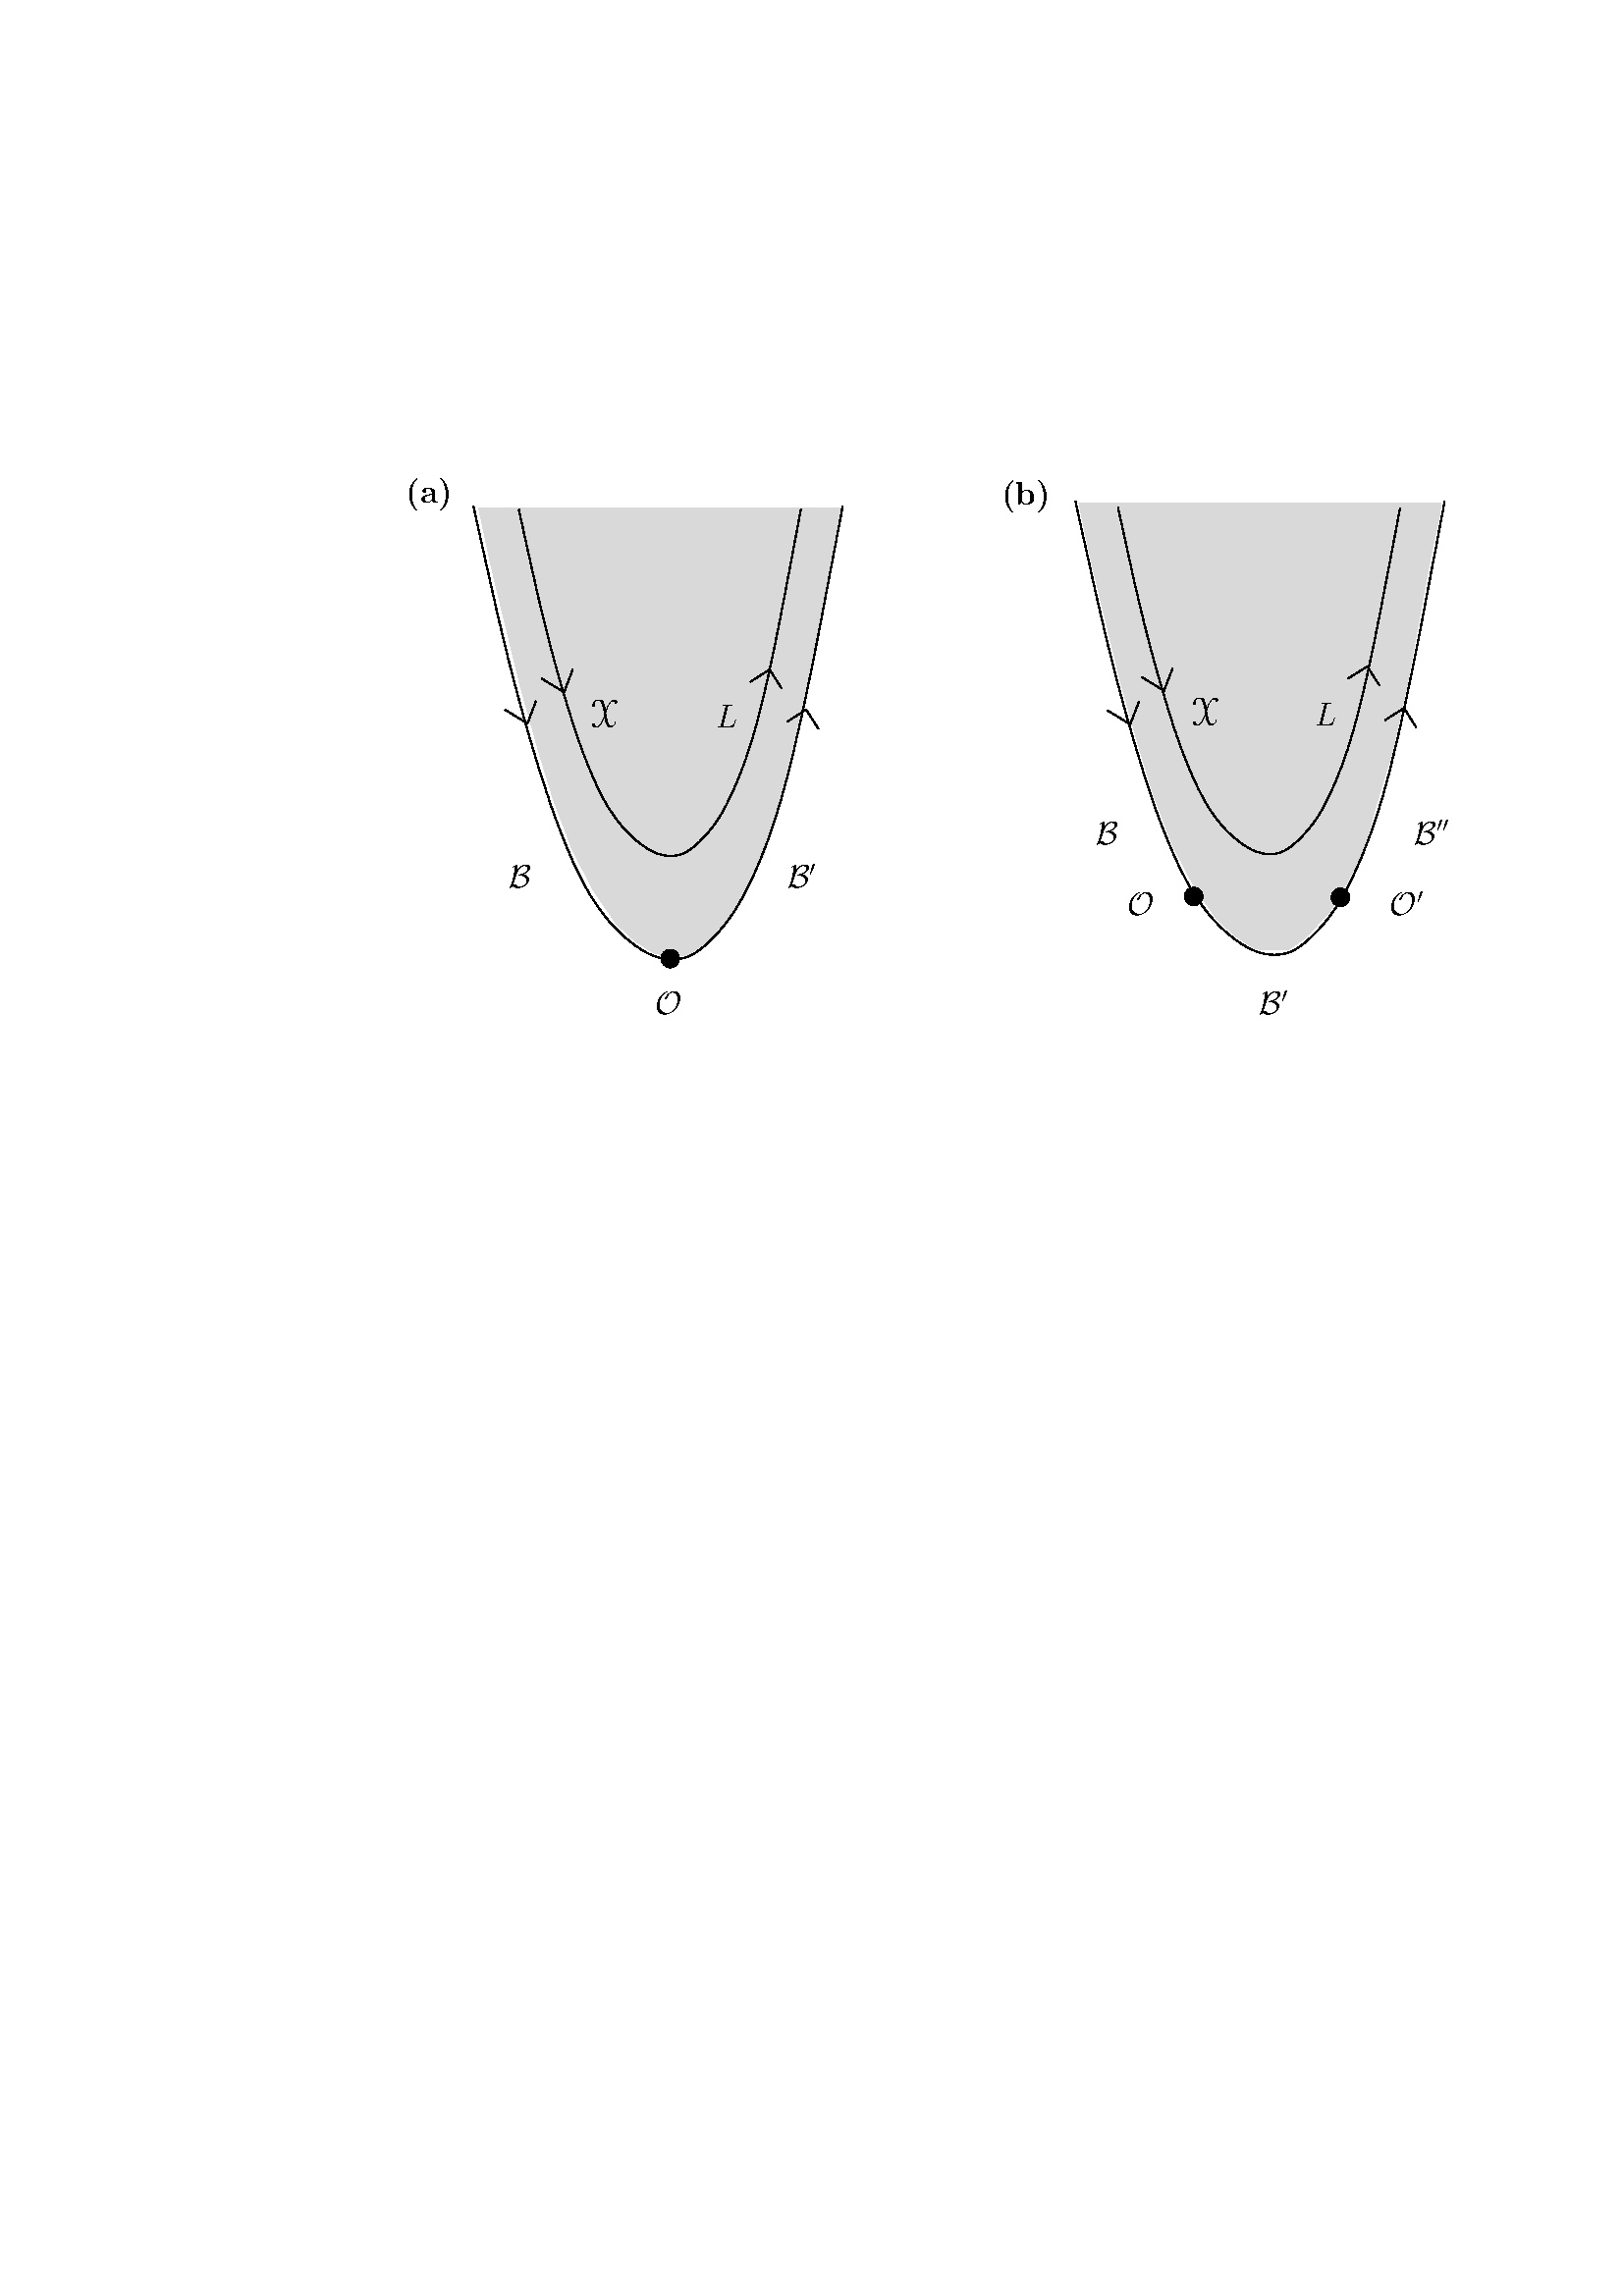
\includegraphics[width=0.75\linewidth]{figures/gla4-6-5.png}
\caption{(a) A line operator $\EUX$ supported on a line $L$ maps branes ${\cal B}$ and ${\cal B}'$ to branes $\EUX{\cal B}$ and $\EUX{\cal B}'$, and likewise maps $({\cal B},{\cal B}')$ strings to $(\EUX{\cal B},\EUX{\cal B}')$ strings. In the picture, the operator ${\EUO}$ determines a $({\cal B},{\cal B}')$ string, which is mapped by the line operator to an $(\EUX{\cal B},\EUX{\cal B}')$ string. (b) These maps preserve the associativity of open string multiplication.（原文 Fig.~10）}
\label{fig:zingop}
\end{figure}
 Associated with the line
operator $\EUX$ is a natural map $\hat\EUX:{\cal H}_{{\cal
B},{\cal B}'}\to{\cal H}_{\EUX{\cal B},\EUX{\cal B}'}$. The
definition of $\hat \EUX$ should be clear from \zingop(a).  In
this picture, from a microscopic point of view, the operator
${\EUO}$ determines a state in ${\cal H}_{{\cal B},{\cal B}'}$,
but from a macroscopic point of view, as $L$ approaches the
boundary, what we see is a state in ${\cal H}_{\EUX{\cal
B},\EUX{\cal B}'}$.

Precisely if $\EUO$ is a multiple of the identity operator, there
is no distinguished point on the boundary of $\Sigma$ at which
$\EUO$ is inserted, and this is true before or after the line
operator $\EUX$ approaches the boundary. So $\hat\EUX$  maps the
identity in ${\cal H}_{{\cal B},{\cal B}}$ (that is, the open
string state that corresponds to the identity operator ${\EUO}=1$)
to the identity in ${\cal H}_{\EUX{\cal B},\EUX{\cal B}}$. It also
preserves the multiplication of open strings.  Indeed, given three
branes ${\cal B}$, ${\cal B}'$, and ${\cal B}''$, the associative
multiplication ${\cal H}_{{\cal B},{\cal B}'}\otimes{\cal
H}_{{\cal B}',{\cal B}''}\to {\cal H}_{{\cal B},{\cal B}''}$ is
defined by joining open strings as in \dunamp(b), or equivalently
by an operator product expansion of operators inserted on the
boundary, as in \zingop(b). This obviously commutes with bringing
a line operator up to the boundary.  The fancy way to summarize
these statements is to say that the line operator $\EUX$
determines a functor mapping the category of branes to itself.

Line operators as symmetries of the category of branes have been
discussed independently and from a different point of view in
\cite{ref99}.  Their relation to duality
transformations will be discussed elsewhere \cite{ref26}.  For an example of the use
of Wilson-like operators to describe boundary perturbations in two-dimensional
conformal field theory, see section 5.5 of
\cite{ref100}.

\par\medskip{\it Line Operators and Enhanced Supersymmetry}

Special Wilson or 't Hooft operators can have more supersymmetry
than what we have claimed so far.

Let us go back to the definition \eqref{eq:ymop}\ of the supersymmetric
Wilson operator.  It is a function of ${\cal
A}_\mu=A_\mu+i\phi_\mu$, so it is invariant under any
supersymmetry that leaves $A_\mu+i\phi_\mu$ invariant. According
to the microscopic formula \eqref{eq:hygo}\ for the transformation of the
fields under supersymmetry, the variation of $A_\mu+i\phi_\mu$
under a supersymmetry generated by an infinitesimal parameter
$\epsilon$ is proportional to
$(\Gamma_\mu+i\Gamma_{\mu+4})\epsilon$.  The condition for
$\epsilon$ to generate a supersymmetry of an arbitrary Wilson line
operator is that this vanishes for $\mu=0,\dots,3$:
% 式 (6.30)
\setcounter{equation}{29}
\begin{equation}\label{eq:pimbo}
\Gamma_{\mu}\Gamma_{\mu+4}\epsilon=i\epsilon,~\mu=0,\dots,3.
\end{equation}

This condition leaves only one unbroken supersymmetry, which is
the one we have exploited so far.

Suppose, however, that $M=\Sigma\times C$ with a product metric.
In this case, the twisting preserves the four supersymmetries that
were characterized in \eqref{eq:zonop}.  Consider also a Wilson operator
defined on a one-manifold ${{\cal S}}$ of the form $\gamma\times
p$ where $\gamma$ is a curve in $\Sigma$ and $p$ is a point in
$C$. For an operator of this type, which we will call a special
Wilson operator, the conditions \eqref{eq:pimbo}\ collapse to
% 式 (6.31)
\setcounter{equation}{30}
\begin{equation}\label{eq:relfo}
\Gamma_{04}\epsilon=\Gamma_{15}\epsilon=i\epsilon.
\end{equation}

These imply the second condition in \eqref{eq:zonop}, and the combined set
of conditions leaves two unbroken supersymmetries.

We can easily see what the extra supersymmetry means.  Special
Wilson operators do not depend on $\varphi$, so they are invariant
under the ${\cal U}_1$ symmetry introduced in section 第~\ref{sec:mhhyper}~节,
which acts on the Higgs field by $\varphi\to\lambda\varphi$,
$|\lambda|=1$. This symmetry rotates complex structure $J$ to
complex structure $K$, so it maps the $B$-model in complex
structure $J$ to the $B$-model in complex structure $K$.  Hence
the two supersymmetries are the topological supercharge of the
$B$-models in complex structures $J$ and $K$.  The topological
supercharge of the $B$-model in any of the complex structures
$I_w$ is a linear combination of these.  So it follows that a
special Wilson operator is what we might call a line operator of
type $(B,B,B)$, that is, it preserves the topological
supersymmetry of the $B$-model in every complex structure of
$\MH$.

We can reason in the same way for special 't Hooft operators, that
is 't Hooft operators supported on a curve ${{\cal S}}$ of the
same type. Special 't Hooft operators are again independent of
$\varphi$ and so invariant under the group ${\cal U}_1$.  This
group rotates the $A$-model in complex structure $K$ into the
$A$-model in complex structure $J$.  General 't Hooft operators
preserve the $A$-type supersymmetry in complex structure $K$, so
special ones do so also in complex structure $J$.  The topological
supercharge of the $B$-model in complex structure $I$ is a linear
combination of those for the $A$-models in complex structures $J$
and $K$.  So actually, the special 't Hooft operators are of type
$(B,A,A)$, that is, they preserve the indicated topological
supersymmetries for complex structures $I$, $J$, and $K$.

This is completely in accord with expectations.  The
$S$-transformation maps Wilson operators to 't Hooft operators,
and as one can see from Table 2 of section 第~\ref{sec:somespec}~节, maps
supersymmetry of type $(B,B,B)$ to supersymmetry of type
$(B,A,A)$.

One can further specialize this situation by taking the metric on
$\Sigma$ to be flat and ${{\cal S}}$ to be a straight line.  In
this case, the line operator describes a static external electric
or magnetic charge.  A Wilson or 't Hooft operator of this form
actually preserves four supersymmetries. For example, for a Wilson
operator supported on a straight line that runs in the time
direction, the conditions for an unbroken supersymmetry reduce to
$\Gamma_{04}\epsilon=i\epsilon$ and
$\Gamma_{2367}\epsilon=\epsilon$.  This system is physically
sensible (if we interpret it with Lorentz signature); it is
described by a real, positive-definite Hilbert space with a
positive-definite, hermitian Hamiltonian $H$. The four unbroken
supersymmetries are the two topological supercharges $Q_i$,
$i=1,2$ described earlier, and their hermitian adjoints
$Q^\dagger_i$.  They obey a physical supersymmetry algebra
$\{Q_i,Q^\dagger_j\}=2\delta_{ij}H$,
$\{Q_i,Q_j\}=0=\{Q^\dagger_i,Q^\dagger_j\}$, for $i,j=1,2$.
